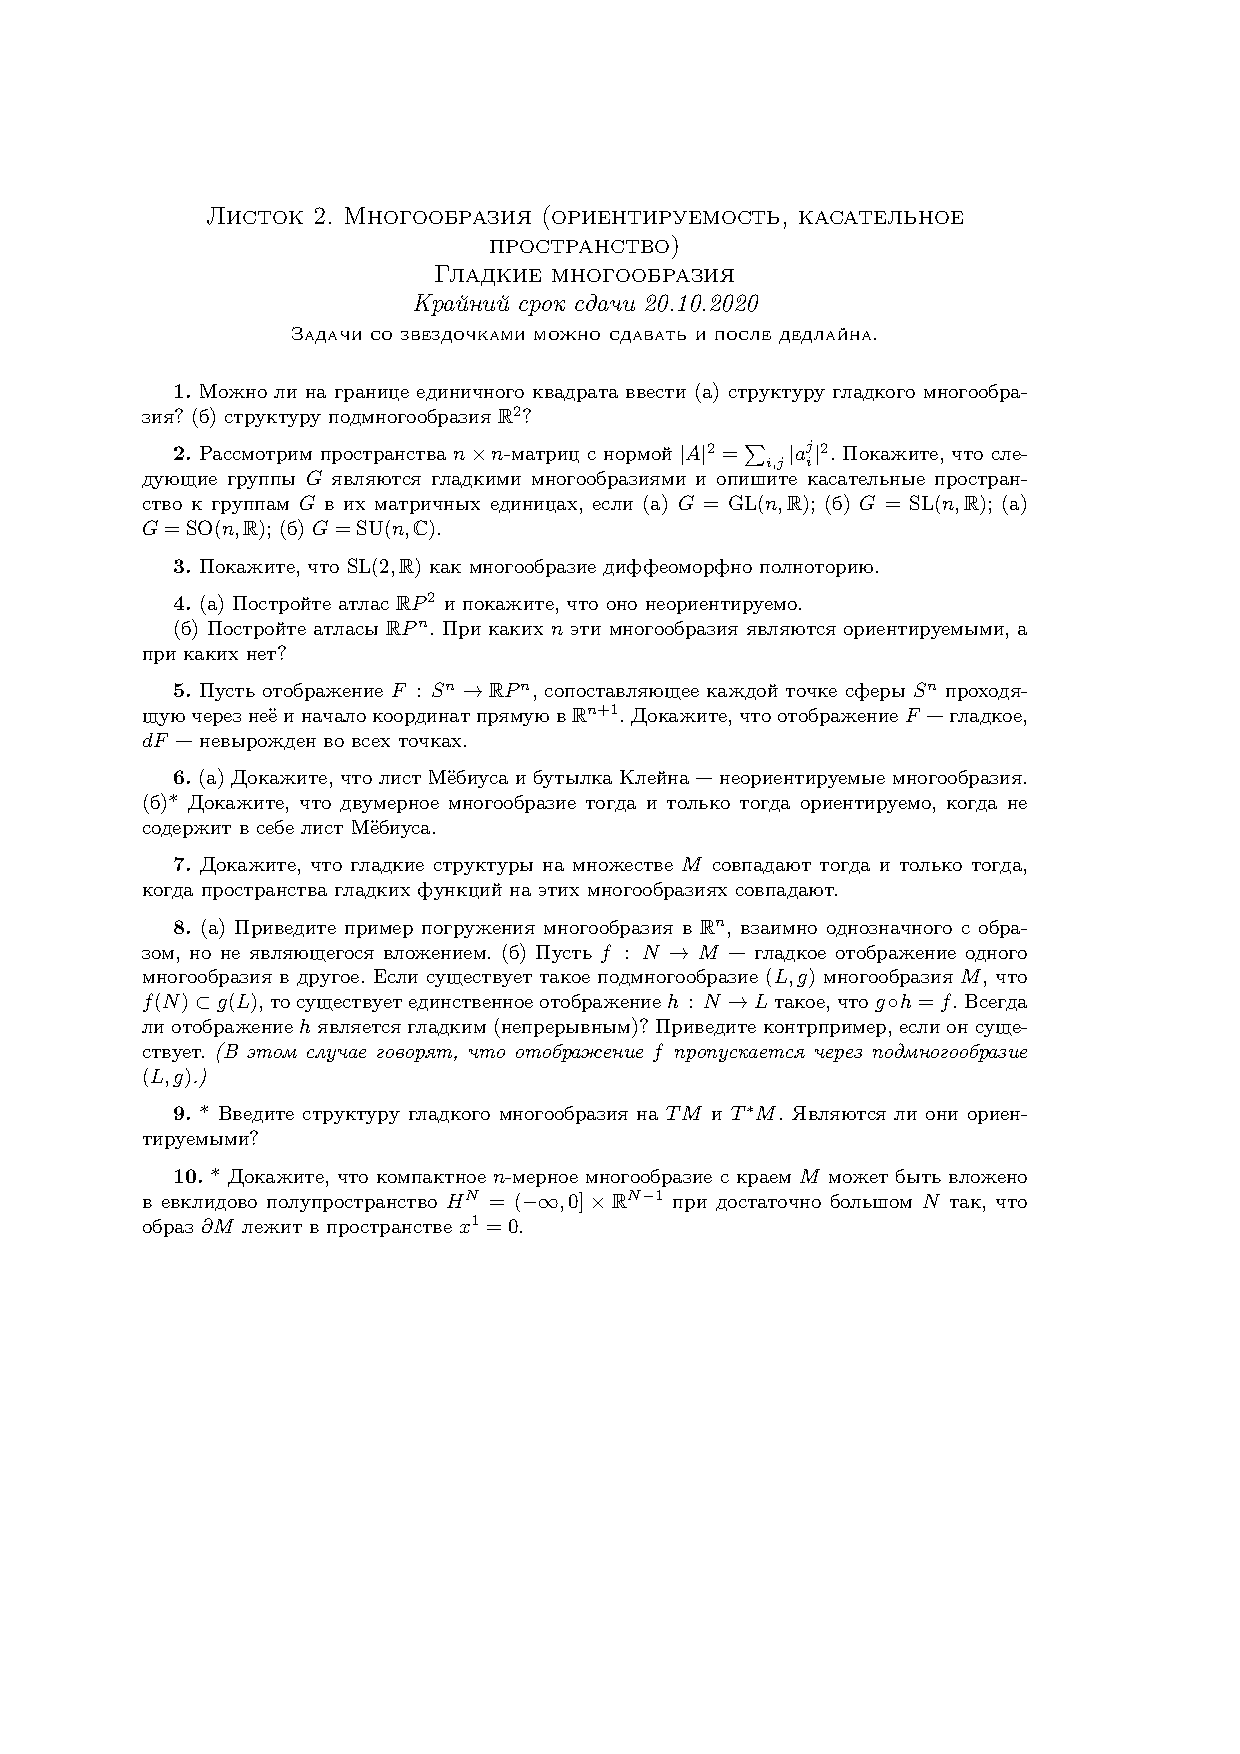
\includepdf[scale=0.95,pages=1,pagecommand=\section*{Условия}]{Tasks/Probl-manif2}
\newpage
\section*{Решения}
\subsection*{Задача 1}
\begin{enumerate}
\item[(а)]
	На границе квадрата существует структура гладкого многообразия.\\
	Так как квадрат $M$ -- 2-мерное гладкое многообразие, то край $\partial M$ -- 1-мерное гладкое многообразие без края\\
	Заметим что можно посмотроить отображение квадрата в окружность
	\begin{gather*}
		f: (x,y) \to \left(x \sqrt{1 - \frac{y^2}{2}}, y \sqrt{1 - \frac{x^2}{2}}\right)
	\end{gather*}
	И окружности в квадрат
	\begin{gather*}
		g: (x,y) \to \\
		\left(\frac{1}{2}\sqrt{2+x^2 - y^2 + 2x\sqrt{2}}) - \frac{1}{2}\sqrt{2 + x^2 - y^2 - 2x\sqrt{2}}, \frac{1}{2}\sqrt{2-x^2 + y^2 + 2y\sqrt{2}}) - \frac{1}{2}\sqrt{2 - x^2 + y^2 - 2y\sqrt{2}}\right)
	\end{gather*}
	Осталось заметить, что $f \circ g = \operatorname{id}_1$ и $g \circ f = \operatorname{id}_2$, а следовательно мы можем взять карты из окружности и отобразить их в квадрат.
\item[(б)]
	Пусть $X = \{(x,y):\ \max(|x|,|y|) = 1\}$ -- квадрат, предположим что это подмногообразие $\mathbb{R}^2$. Пусть $v$ -- его вершина (любая), тогда касательное пространство к $X$ в $v$ должно иметь размерность $1$, но $T_v X$ имеет размерность $0$ -- противоречие.
	\vskip 0.1in
	Подмногообразие размерности $0$ -- дискретно, а размерности $2$ -- локально открыто, но так как $X$ не является ни тем, ни другим, то оно имеет размерность $1$.\\
	Гладкая кривая на $X$, проходящая через $v$ при $t = 0$, должна иметь $0$ производную в $t = 0.$
\end{enumerate}


\subsection*{Задача 2}
\begin{enumerate}
\item[(а)]
	$G = GL_n(\mathbb{R})$, атлас $(G, \varphi = \det)$\\
	$GL_n(\mathbb{R})$ -- открытое множество в $\mathbb{R}^{n^2}$, так как дополнение при непрерывном отображении $\det: G \to \mathbb{R}$ замкнуто\\
	Прообраз $\mathbb{R} \backslash \{0\}$ (то есть $G$) открыт в $\mathbb{R}^{n^2}$, следовательно $G$ -- многообразие
	\vskip 0.2in
	Гладким путем из точки $p$ называется гладкое отображение $\gamma: (-\varepsilon, \varepsilon) \to M, \quad \gamma(0) = p$\\
	Пути эквивалентны, если $\frac{d}{dt} \varphi(\gamma_1(t)) |_{t = 1} = \frac{d}{dt} \varphi(\gamma_2(t))|_{t = 0}$
	\vskip 0.2in
	Касательное пространство к $G$ в $E$:\\
	$A \in T_E G\ \leftrightarrow \exists$ гладкое отображение $\gamma: (\-\varepsilon, \varepsilon) \to G$, $\gamma(0) = E,\ \dot{\gamma}(0) = A$\\
	Проверим, что подходит $\gamma(t) = E + tA$
	\begin{gather*}
		\det E = 1 \ne 0\ \rightarrow \exists \varepsilon >0:\ \sqrt{\sum||b_{ij}||^2} = ||B|| < \varepsilon\quad \det(B+E) \ne 0\\
		\forall A \in \operatorname{Mat}_{n \times n}(\mathbb{R})\quad \exists \delta > 0:\ \forall t \in (-\delta, \delta):\ \det(E + tA) \ne 0\\
		\gamma(-\varepsilon, \varepsilon) \in G
	\end{gather*}
	
\begin{comment}
	$GL_n(\mathbb{R}) = \{A \in \operatorname{Mat}_{n\times n}(\mathbb{R})| \det A \ne 0\}$ -- открытое подмножество $\mathbb{R}^{n^2}$:\\
	Определитель матрицы $A$ -- многочлен от коэф. матрицы, непрерывная функция. Тогда, так как $|A| \ne 0$, $A \to \det A$ непрерывное отображение, то есть $\{A\ |\ |A| \ne 0\} \to \mathbb{R}\backslash\{0\}$.\\
	$\mathbb{R}\backslash \{0\}$ открыто, отображение непрерывно, значит прообраз открытого открыт, откуда $\{A\ |\ |A| \ne 0\} \subset \mathbb{R}^{n^2}$ -- открыто в $\mathbb{R}^{n^2}$.\\
	Тогда карта одна и отображение тождественное, а следовательно и гладкое
	\vskip 0.2in
	Касательное пространство:\\
	$\dim TGL_n(\mathbb{R}) = \dim GL_n(\mathbb{R}) = n^2$ и $GL_n(\mathbb{R}) \subset \mathbb{R}^{n^2}$, следовательно касательное пространство является подпространством $\mathbb{R}^{n^2}$, но если размерность подпространства = размерности пространства, то подпространство = пространству, то есть $TGL_n(\mathbb{R}) = \operatorname{Mat}_n(\mathbb{R})$
\end{comment}
	
\item[(б)]
	$SL_n(\mathbb{R}) = \{A \in \operatorname{Mat}_{n \times n}(\mathbb{R})\ |\ \det A = 1\}$\\
	Покажем, что $SL_n(\mathbb{R})$ -- подмногообразие $\mathbb{R}^n$. Знаем, что $M \subset \mathbb{R}^n$ размерности $k$, если $M$ локально задано в виде нулей гладкой функции $F$, ранга $n-k$\\
	Пусть $G: \operatorname{Mat}_{n \times n}(\mathbb{R}) \to \mathbb{R}: A \mapsto \det A - 1$. Тогда $SL_n(\mathbb{R}) = \{A \in \operatorname{Mat}_{n \times n}(\mathbb{R}) = \{A \in \operatorname{Mat}_{n \times n}(\mathbb{R})\ |\ G(A) = 0\}\}$, $\dim (SL_n(\mathbb{R})) = n^2 - 1$, следовательно нужно показать, что ранг $J_{G} = n^2 - n^2 + 1 = 1$
	\begin{gather*}
	J_{G} = 
	\begin{pmatrix}
		\frac{\partial G}{\partial x_{1\ 1}} \\ \vdots \\ \frac{\partial G}{\partial x_{n\ n}}
	\end{pmatrix}
	\end{gather*}
	Эта матрица ранга 1 или 0 (если $J_{G} = 0$). Докажем, что $J_{G} \ne 0$, то есть все частные производные ненулевые\\
	$\det A = \sum\limits_{n = 1}^{n} (-1)^{i+1} a_{i\ 1} M_{i\ 1}$ -- разложим по первому столбцу.\\
	Рассмотрим $(-1)^{i+1} M_{i\ 1}$, $M_{i\ 1}$ -- определитель матрицы, полученной вычеркиванием $i$ строки и $1$ столбца, пусть $J_{G} = 0$, то есть все частные производные нулевые, тогда миноры нулевые, в следовательно $\det A = 0$, но $\det A = 1$.\\
	В индуцированной топологии из $\mathbb{R}^n$ подмногообразие является многообразием по определению.
	\vskip 0.2in
	Касательное пространство:
	\begin{gather*}
		\gamma(t): (-\varepsilon, \varepsilon) \to SL_n(\mathbb{R})\\
		\gamma(t) = E + \dot{\gamma}t + \overline{\overline{o}}(t)\\
		1 = \det \gamma(t) = \det (E + \dot{\gamma}(0)t + \overline{\overline{o}}(t)) = \det(E + t \dot{\gamma} + \overline{\overline{o}}(t)) = \\
		= 1 + t \frac{d}{dt} (\det (E + t \dot{\gamma}(0))) + \overline{\overline{o}}(t) = 1 + t \cdot \operatorname{tr} \dot{\gamma}(0) + \overline{\overline{o}}\\
		\sum\limits_{i,j} \frac{\partial \det}{\partial a_{ij}} |_{E} \dot{\gamma}(0)_{ij} = \sum\limits_{i,j} A_{ij}|_{E} \dot{\gamma}(0)_{ij} = \sum \delta_{ij} \dot{\gamma}(0)_{ij} = \sum\limits_{i} \dot{\gamma}(0)_{ii} = \operatorname{tr} \dot{\gamma}(0)\quad (A_{ij} \text{ -- алгебраическх дополнений})\\
		t \cdot \operatorname{tr} \dot{\gamma}(0) + \overline{\overline{o}} = 0\\
		\operatorname{tr} \dot{\gamma}(0) = 0\\
		T_E SL_n (\mathbb{R}) \subset \{\text{матрицы} A|\ \operatorname{tr}A = 0\}\text{, но размерность этих множеств: } n^2 - 1\\
		T_E SL_n (\mathbb{R}) = \{\text{матрицы с нулевым следом}\}
	\end{gather*}
\item[(в)]
	$SO_n(\mathbb{R}): AA^t = E$\\
	Аналогично прошлому пункту покажем, что $O_n(\mathbb{R})$ -- подмногообразие $\mathbb{R}^{n^2}$ (функция, нулями которой является $O_n(\mathbb{R})$, -- $F(A) = A^{t}A - E$). Рассмотрим $\{A|\ \det A > 0,\ A \in O_n(\mathbb{R})\}$ -- это $SO_n(\mathbb{R})$, открыто в $O_n(\mathbb{R})$, следовательно многообразие
	\begin{gather*}
		\gamma(t) = (-\varepsilon, \varepsilon) \to SO_n(\mathbb{R})\\
		\gamma(t) = E + \dot{\gamma}t + \overline{\overline{o}}(t)\\
		(\gamma(t))^t = E + (\dot{\gamma}(0))^t t + \overline{\overline{o}}(t)\\
		(E + \dot{\gamma}(0)t + \overline{\overline{o}})(E + (\dot{\gamma})^t t + \overline{\overline{o}}(t)) = E + \dot{\gamma}(0)t + (\dot{\gamma}(0))^t t + \overline{\overline{o}}(t) = E\\
		\dot{\gamma}(0)t + (\dot{\gamma}(0))^t t + \overline{\overline{o}}(t) = 0\\
		\dot{\gamma}(0) = -(\dot{\gamma}(0))^t\\
		T_E SO_n(\mathbb{R}) \text{ -- кососсимметричные матрицы}
	\end{gather*}
\item[(г)]
	$SU_n(\mathbb{C}):\ AA^{\star} = A^{\star}A = E,\ A^{\star} = \overline{A^{t}}$ Аналогично прошлому пункту это многообразие
	\begin{gather*}
		(E + \dot{\gamma}t + \overline{\overline{o}}(t))(E + \overline{(\dot{\gamma}(0))^t}t + \overline{\overline{o}}(t)) =
		E + \dot{\gamma}(0)t + \overline{(\dot{\gamma}(0))^t} t + \overline{\overline{o}}(t) = E\\
		\dot{\gamma}(0) = -\overline{(\dot{\gamma}(0))^t}
	\end{gather*}
	Следовательно $T_E SU_n(\mathbb{C})$ -- косоэрмитовы матрицы
\end{enumerate}

\newpage
\subsection*{Задача 3}
	$K \times A \times N \to SL(2,\mathbb{R})$ -- непрерывно и сюръективно
	\begin{gather*}
		K = 
		\Bigg\{
		\begin{pmatrix}
		\cos(\theta) & -\sin(\theta)\\
		\sin(\theta) & \cos(\theta)
		\end{pmatrix}
		\Bigg\}\\
		A = 
		\Bigg\{
		\begin{pmatrix}
		r & 0 \\ 0 & \frac{1}{r}
		\end{pmatrix}
		:\ r > 0
		\Bigg\}\\
		N = 
		\Bigg\{
		\begin{pmatrix}
		1 & x \\ 0 & 1
		\end{pmatrix}
		\Bigg\}
	\end{gather*}
	Теорема:\\
	$\forall g \in SL(2,\mathbb{R})\ \exists!\ k \in K, a \in A, n \in N:\ g = kan$
	\vskip 0.2in
	Рассмотрим базис $(e_1,e_2)$ плоскости $\mathbb{R}^2$\\
	$g = \begin{pmatrix} a & b \\ c & d \end{pmatrix}$ ($ad - bc = 1$) тогда $ge_1 = \begin{pmatrix} a \\ c \end{pmatrix}$ и $ge_2 = \begin{pmatrix} b & d \end{pmatrix}$ -- тоже базис, так как лнз\\
	\begin{figure}[!h]
		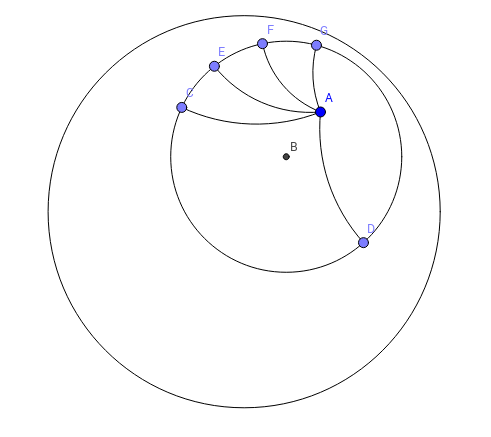
\includegraphics[width=0.2\linewidth]{pic8}
	\end{figure}
	$|g| = 1 > 0$, а следовательно ориентация $ge_1, ge_2$ та же, следовательно и у $\rho_{-\theta}(ge_1), \rho_{-\theta}(ge_2)$ та же, откуда $\rho_{\theta}(ge_2)$ в верхней полуплоскости.\\
	Если $\rho_{-\theta}(ge_1) \in \left[Ox\right)$, то $\rho_{-\theta}(ge_1) = le_1$\\
	$l$ -- длина $\rho_{-\theta}(ge_1)$, то есть $l = \sqrt{a^2 + c^2}$\\
	Умножение на $\begin{pmatrix} \frac{1}{l} & 0 \\ 0 & l \end{pmatrix}$ даст $\rho_{-\theta}(ge_1) \to e_1$, так как
	\begin{gather*}
		\rho_{-\theta}(ge_1) = 
		\begin{pmatrix}
			l \\ 0
		\end{pmatrix}\\
		\begin{pmatrix}
			\frac{1}{l} & 0\\
			0 & l
		\end{pmatrix}
		\begin{pmatrix}
			l \\ 0
		\end{pmatrix}
		=
		\begin{pmatrix}
			1 \\ 0
		\end{pmatrix}
		=
		e_1
	\end{gather*}
	$\begin{bmatrix}
		\frac{1}{l} & 0\\
		0 & l
	\end{bmatrix}
	= 1 > 0$, следовательно вектор 
	$\begin{pmatrix} \frac{1}{l} & 0 \\ 0 & l \end{pmatrix} \rho_{-\theta}(ge_2)$ снова лежит в верхней полуплоскости\\
	$s(e_1,e_2) = 1,\ s(ge_1,ge_2) = 1$ так как $|g| = 1,\ s(\rho_{-\theta}(ge_1),\rho_{-\theta}(ge_2)) = 1$ (поворот)
	\begin{gather*}
		s(\begin{pmatrix} \frac{1}{l} & 0 \\ 0 & l \end{pmatrix} \rho_{-\theta}(ge_1),
		\begin{pmatrix} \frac{1}{l} & 0 \\ 0 & l \end{pmatrix} \rho_{-\theta}(ge_2))
		=
		s(e_1,
		\begin{pmatrix} \frac{1}{l} & 0 \\ 0 & l \end{pmatrix}\rho_{-\theta}(ge_2)) = 1\\
		\begin{pmatrix} \frac{1}{l} & 0 \\ 0 & l \end{pmatrix}\rho_{-\theta}(ge_2) = \begin{pmatrix} x \\ 1 \end{pmatrix}
	\end{gather*}
	Осталось перевести $\begin{pmatrix} x \\ 1 \end{pmatrix}$ в $e_2 = \begin{pmatrix} 0 \\ 1 \end{pmatrix}$ так что $e_1$ останется на месте.
	\begin{gather*}
		\begin{pmatrix}
			1 & -x\\
			0 & 1
		\end{pmatrix}
		\begin{pmatrix}
			x \\ 1
		\end{pmatrix}
		=
		\begin{pmatrix}
			0 \\ 1
		\end{pmatrix}
		=
		e_2\\
		\begin{pmatrix}
			1 & -x\\
			0 & 1
		\end{pmatrix}
		\begin{pmatrix}
			1 \\ 0
		\end{pmatrix}
		=
		\begin{pmatrix}
			1 \\ 0
		\end{pmatrix}
		=
		e_1
	\end{gather*}
	Откуда получаем
	\begin{gather*}
		\begin{pmatrix}
			1 & -x\\
			0 & 1
		\end{pmatrix}
		\begin{pmatrix}
			\frac{1}{e} & 0\\
			0 & e
		\end{pmatrix}
		\rho_{-\theta}g
		=
		\begin{pmatrix}
			1 & 0\\
			0 & 1
		\end{pmatrix}\\
		g = (\rho_{-\theta})^{-1}
		\begin{pmatrix}
			\frac{1}{l} & 0\\
			0 & l
		\end{pmatrix}^{-1}
		\begin{pmatrix}
			1 & -x\\
			0 & 1
		\end{pmatrix}^{-1}
		\begin{pmatrix}
			1 & 0\\
			0 & 1
		\end{pmatrix}
		=
		\rho_{\theta}
		\begin{pmatrix}
			l & 0\\
			0 & \frac{1}{l}
		\end{pmatrix}
		\begin{pmatrix}
			1 & x\\
			0 & 1
		\end{pmatrix}
	\end{gather*}
	Откуда
	\begin{gather*}
		g = 
		\begin{pmatrix}
			\cos(\theta) & -\sin(\theta)\\
			\sin(\theta) & \cos(\theta)
		\end{pmatrix}
		\begin{pmatrix}
			l & 0\\
			0 & \frac{1}{l}
		\end{pmatrix}
		\begin{pmatrix}
			1 & x\\
			0 & 1
		\end{pmatrix}
	\end{gather*}
	Проверим что представление единственно
	\begin{gather*}
		\begin{pmatrix}
			l\cos(\theta) & xl\cos(\theta)-\frac{1}{l}\sin(\theta)\\
			l\sin(\theta) & xl\sin(\theta)+\frac{1}{l}\cos(\theta)
		\end{pmatrix}
		=
		\begin{pmatrix}
			a & b \\ c & d
		\end{pmatrix}\\
		a^2 + c^2 = l^2\cos^2 \theta + l^2 \sin^2 \theta\\
		l = \sqrt{a^2 + c^2}\\
		\cos(\theta) = \frac{a}{l}\\
		\sin(\theta) = \frac{c}{l}\\
		\\
		\begin{cases}
			xl \frac{a}{l} - \frac{1}{l} \frac{c}{l} = b\\
			xl \frac{c}{l} + \frac{1}{l} \frac{a}{l} = d
		\end{cases}\\
		\begin{cases}
			ax = \frac{bl^2 + c}{l^2}\\
			cx = \frac{dl^2 - a}{l^2}
		\end{cases}\\
		\begin{cases}
			x = \frac{b(a^2 + c^2) + c}{(a^2 + c^2)a}\\
			x = \frac{d(a^2 + c^2) - a}{(a^2 + c^2)c}
		\end{cases}\\
		ad - bc = 1\\
		bc^2 + c = c(bc + 1) = cad\\
		x = \frac{a^2b + cad}{a(a^2 + c^2)} = \frac{ab + cd}{a^2 + c^2}
	\end{gather*}
	Заметим, что $a^2 + c^2 \ne 0$ так как $a \ne 0$ или $c \ne 0$, а следовательно $x$ однозначно определен.
	\vskip 0.3in
	
	$K \times A \times N$ диффеоморфно $SL(2,\mathbb{R})$
	\begin{gather*}
		f: K \times A \times N \to SL(2,\mathbb{R})\\
		f:(k,a,n) \to kan
	\end{gather*}
	По теореме $f$ биективно и $\exists f^{-1}$
	\begin{gather*}
		k(g) = 
		\begin{pmatrix}
			\frac{a}{l(g)} & -\frac{c}{l(g)}\\
			\frac{c}{l(g)} & \frac{a}{l(g)}
		\end{pmatrix}\\
		a(g) = 
		\begin{pmatrix}
			l(g) & 0\\
			0 & \frac{1}{l(g)}
		\end{pmatrix}\\
		n(g) = 
		\begin{pmatrix}
			1 & \frac{ab + cd}{a^2 + c^2}\\
			0 & 1
		\end{pmatrix}
	\end{gather*}
	$K \simeq S^{1}$ так как определяется углом $\theta$\\
	$A \simeq \mathbb{R}_{>0} \simeq \mathbb{R}$ определяется числом $l > 0$\\
	$N \simeq \mathbb{R}$ определяется числом $x$\\
	Следовательно $SL(2,\mathbb{R}) \simeq S^{1} \times \mathbb{R}^{2}$ и $\mathbb{R}^2 \simeq D^{1}$
	\begin{gather*}
		(x,y) \to (\frac{x}{\sqrt{1 + x^2 + y^2}}, \frac{y}{\sqrt{1 + x^2 + y^2}})
	\end{gather*}
	Тогда $SL(2,\mathbb{R}) \simeq S^{1} \times D^{1}$ -- полноторий



\subsection*{Задача 4}
\begin{enumerate}
\item[(а)]
	Зададим структуру гладкого многообразия на проективной плоскости $\mathbb{R}P^2$. Будем представлять ее как множество прямых в $\mathbb{R}^3$, проходящих через начало координат. Каждая прямая определена вектором с координатами $(x,y,z)$ (и пропорциональные вектора задают одну и ту же прямую). Рассмотрим атлас из 3 карт $(U_1, \varphi_1), (U_2, \varphi_2), (U_3, \varphi_3)$, где $U_1 = \{(x,y,z)\|\ x \ne 0\}, U_2 = \{(x,y,z)\|\ y \ne 0\}, U_3 = \{(x,y,z)\|\ z \ne 0\}, \varphi_1(x,y,z) = (\frac{y}{x}, \frac{z}{x}), \varphi_2(x,y,z) = (\frac{x}{y}, \frac{z}{y}), \varphi_3(x,y,z) = (\frac{x}{z}, \frac{y}{z})$. Тогда можно заметить, что полученное множество прямых можно рассматривать как диск с отождествленными диаметрально противоположными точками, тогда, если взять диаметр полученного диска и рассмотреть какую-то его окрестность, то полученное множество будет летой мебиуса, а она неориентируема.
	
\item[(б)]
	\begin{gather*}
		\mathbb{R}P^n: (x_0,\ldots,x_n) \sim (\lambda x_0,\ldots,\lambda x_n)\quad \forall \lambda \ne 0\\
		U_i = \{(x_0, \ldots, x_n)|\ x_i \ne 0\}\quad i = 0,\ldots,n\\
		\varphi_i: U_i \to \mathbb{R}^n,\ (x_0,\ldots,x_n) \to \left(\frac{x_0}{x_i},\ldots,\frac{x_{i-1}}{x_i},\frac{x_{i-1}}{x_i},\ldots,\frac{x_n}{x_i}\right)
	\end{gather*}
	Пусть $a = (a_0,\ldots,a_{i-1},a_{i+1},\ldots,a_n)$
	\begin{gather*}
		\varphi_i^{-1}(a) = (a_0,\ldots,a_{i-1},1,a_{i+1},\ldots,a_n)\\
		\varphi_j \circ \varphi_i^{-1}(a) = \left(\frac{a_0}{a_j},\ldots,\frac{a_{i-1}}{a_j},\frac{1}{a_j},\frac{a_{i+1}}{a_j},\ldots,\frac{a_{j-1}}{a_j},\frac{a_{j+1}}{a_j},\ldots,\frac{a_n}{a_j}\right) \text{ -- диффеоморфизм}
	\end{gather*}
	Посчитаем якобиан
	\begin{gather*}
		J_{ij} =
		\begin{pmatrix}
			\frac{1}{a_j} & 0 & 0 & -\frac{a_0}{a_j^2} & 0 &&&&& 0\\
			0 & \ddots & 0 & \vdots & 0 &&&&& 0\\
			0 & 0 & \frac{1}{a_j} & -\frac{a_{j-1}}{a_j^2} & 0 &&&&& 0\\
			0 && 0 & -\frac{a_{j+1}}{a_j^2} & \frac{1}{a_j} & 0 &&&& 0\\
			0 && 0 & \vdots & 0 & \ddots & 0 &&& 0\\
			0 && 0 & -\frac{a_{i-1}}{a_j^2} & 0 & 0 & \frac{1}{a_j} & 0 && 0\\
			0 && 0 & -\frac{1}{a_j^2} & 0 & 0 & 0 & 0 & 0 & 0\\
			0 && 0 & -\frac{a_{i+1}}{a_j^2} & 0 && 0 & \frac{1}{a_j} & 0 & 0\\
			0 && 0 & \vdots & 0 &&& 0 & \ddots & 0\\
			0 && 0 & -\frac{a_n}{a_j^2} & 0 &&&& 0 & \frac{1}{a_j}
		\end{pmatrix}\\
		\det(J_{ij}) = -\frac{1}{a_j^n} (-1)^{i-j} = (-1)^{|i-j| - 1} \cdot -\frac{1}{a_j^{n+1}} = (-1)^{|i-j|} \frac{1}{a_j^{n+1}}
	\end{gather*}

	\begin{figure}[!h]
		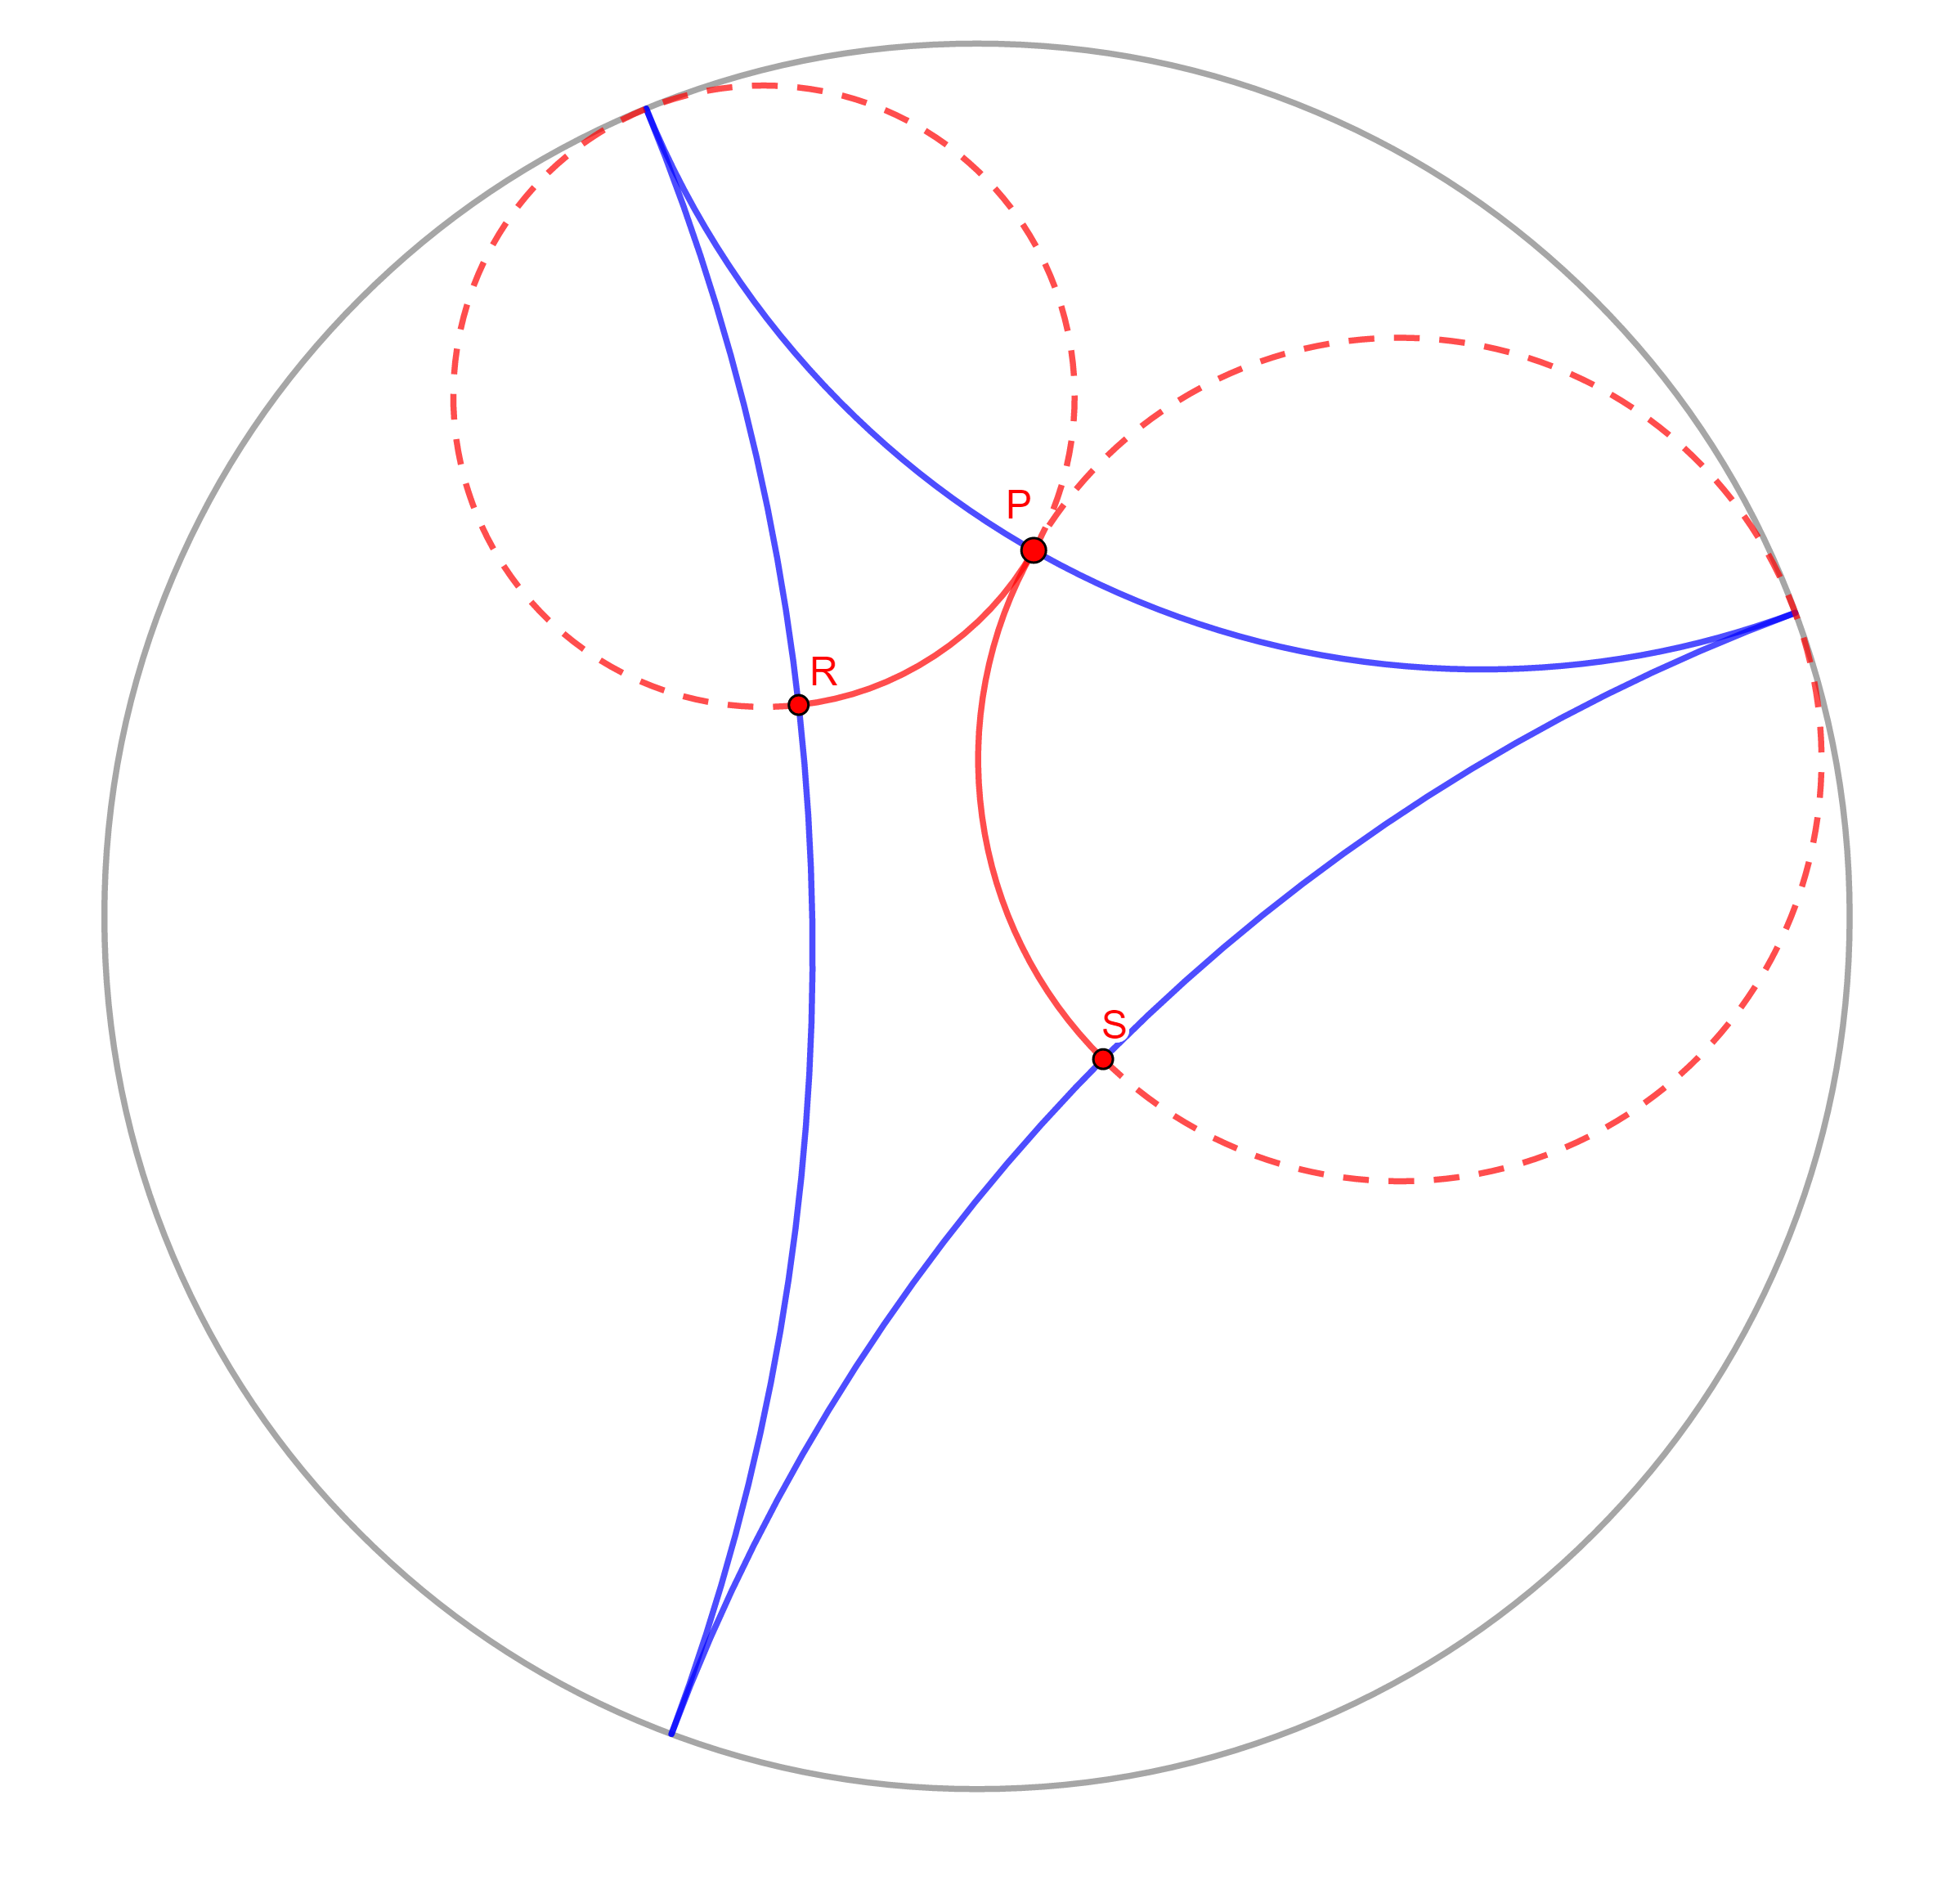
\includegraphics[width=0.55\linewidth]{pic11}
	\end{figure}
	$|i-1-j+1|$ пересечение\\
	$\tilde{U_i} = \{(x_0:\ldots:x_n)|\ \frac{x_{i+1}}{x_i} < 0\}$\\
	Рассмотрим цепочку $\tilde{U_0},\ldots,\tilde{U_n}$\\
	\begin{gather*}
		\tilde{U_i} \cap \tilde{U}_{i+1} = \biggl\{ (x_0:\ldots:x_n)|\ \frac{x_{i+1}}{x_i} < 0,\ \frac{x_{i+2}}{x_{i+1}} < 0\biggr\}
	\end{gather*}
	Следовательно $x_i,x_{i+2}$ одного знака, а $x_{i+1}$ -- другого
	\vskip 0.2in
	По аналогии с 4(а)
	\begin{gather*}
		\varphi_{01}:(x_0,\ldots,x_n) \to (1,x_0,\ldots,x_n) \to \left(\frac{1}{x_0}, \ldots, \frac{x_n}{x_0}\right)\quad (x_0 < 0)\\
		|J_{01}| = (-1) \frac{1}{x_0^{n+1}} > 0\\
		\varphi_{12}: (x_0, \ldots, x_n) \to (x_0, 1, x_1, \ldots, x_n) \to \left(\frac{x_0}{x_1},\ldots,\frac{x_n}{x_1}\right)\quad (x_1 < 0)\\
		|J_{12}| = (-1) \frac{1}{x_1^{n+1}} > 0\\
		\vdots\\
		\varphi_{n0}: (x_0,\ldots,x_n) \to (x_0,\ldots,x_n,1) \to \left(\frac{x_0}{x_n},\ldots,\frac{1}{x_n}\right)\quad (x_n > 0)\\
		|J_{n0}| = (-1) \frac{1}{x_n^{n+1}} < 0
	\end{gather*}
	Следовательно цепочка карт противоречива для четного $n$
	\vskip 0.2in
	Докажем, что $\mathbb{R}P^n$ ориентируемо для нечетного $n$\\
	Заменим $(U_i,\varphi_i)$ на $(U_i,\tilde{\varphi_i})$ для четных $i$
	\begin{gather*}
		\tilde{\varphi_i}: (x_0:\ldots:x_n) \to (-\frac{x_0}{x_i}, \frac{x_1}{x_i},\ldots,\frac{x_{i-1}}{x_i}, \frac{x_{i+1}}{x_i},\ldots,\frac{x_n}{x_i})\\
		\tilde{\varphi_i}^{-1}: (*a_0,a_1,\ldots,a_{i-1},1,a_{i+1},\ldots,a_n)
	\end{gather*}
	Тогда у $\varphi_{ij} = \varphi_j \circ \varphi_i^{-1}$ поменяется знак, если $i,j$ разной четости
	\begin{gather*}
		|J_{ij}| = (-1)^{|i-j|}\frac{1}{x_j^{n+1}}
	\end{gather*}
	Если $i,j$ одной четности, то $(-1)^{|i-j|} = 1$ и $|J_{ij}| > 0$\\
	Если $i,j$ разной четности, то $(-1)^{|i-j| + 1} = 1$ и $|J_{ij}| > 0$\\
	Следовательно атлас ориентирующий для нечетного $n$
\end{enumerate}


\subsection*{Задача 5}
	$F: S^n \to \mathbb{R}P^n\quad (x_0,\ldots,x_n) \to (x_0:\ldots:x_n)$\\
	Атла*с на $S^n$:
	\begin{gather*}
	(U_{K+}, \varphi_{K+}): U_{K+} = \{x \in S^{n}|\ X_K > 0\}\\
	\varphi_{K+}(x) = (x_0,\ldots,x_{k-1},x_{k+1},\ldots,x_n)\\
	(U_{K-}, \varphi_{K-}): U_{K-} = \{x \in S^{n}|x_K < 0\},\ \varphi_{K-}(x) = \varphi_{K+}(x)
	\end{gather*}
	\begin{figure}[!h]
		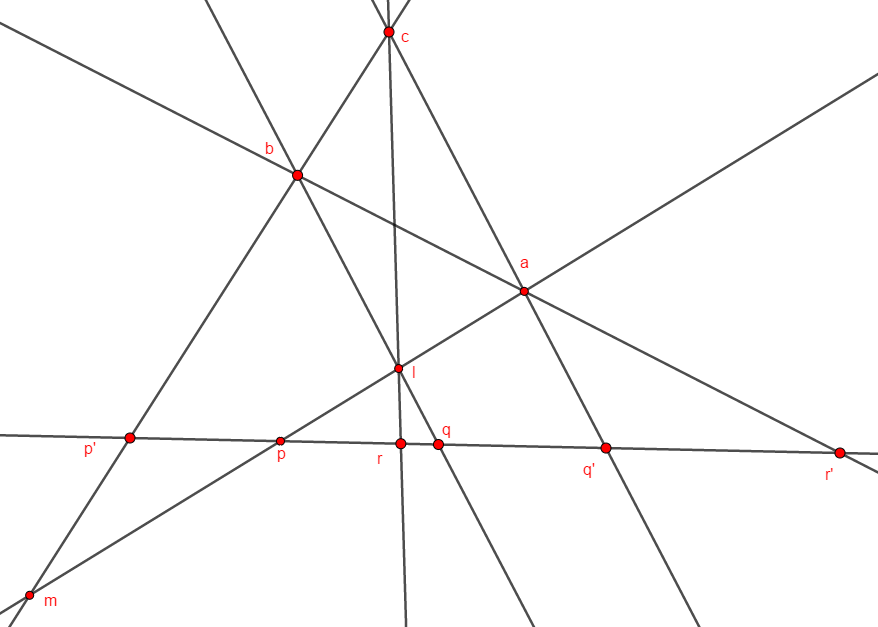
\includegraphics[width=0.55\linewidth]{pic9}
	\end{figure}
	Атлас на $\mathbb{R}P^n$:
	\begin{gather*}
		(V_i, \psi_i):\ V_i = \{x \in \mathbb{R}P^n|\ x_i \ne 0\}\\
		\psi_i(x) = \left(\frac{x_0}{x_i},\ldots,\frac{x_{i-1}}{x_i},\frac{x_{i+1}}{x_i},\ldots,\frac{x_n}{x_i}\right)\\
		\tilde{F} = \psi_i \circ F \circ \varphi_{K\pm}^{-1}
	\end{gather*}
	Пусть $i \ne k$, тогда 
	\begin{gather*}
		\varphi_{K\pm}^{-1}(x_0,\ldots,x_{k-1},x_{k+1},\ldots,x_n) = (x_0,\ldots,x_k,\pm\sqrt{1-||\tilde{x}||^2},x_{k+1},\ldots,x_n)\\
		\tilde{F}(\tilde{x}) = (\frac{x_0}{x_i},\ldots,\frac{x_{i-1}}{x_{i+1}}, \ldots, \frac{x_{k-1}}{x_i}, \frac{\pm\sqrt{1-||\tilde{x}||^2}}{x_i},\frac{x_{k+1}}{x_i},\ldots,\frac{x_n}{x_i}) = \tilde{y}\\
		\tilde{F}^{-1}(\tilde{y}) = \\
		\left(\pm\frac{y_0}{\sqrt{1+||\tilde{y}||^2}}, \ldots, \pm\frac{y_{i-1}}{\sqrt{1+||\tilde{y}||^2}}, \pm\frac{1}{\sqrt{1+||\tilde{y}||^2}}, \pm\frac{y_{i+1}}{\sqrt{1+||\tilde{y}||^2}}, \ldots, \pm\frac{y_{k-1}}{\sqrt{1+||\tilde{y}||^2}}, \pm\frac{y_{k+1}}{\sqrt{1+||\tilde{y}||^2}}, \ldots, \pm\frac{y_n}{\sqrt{1+||\tilde{y}||^2}}\right)
	\end{gather*}
	Пусть $i = k$, тогда
	\begin{gather*}
		\tilde{F}(\tilde{x}) = \left(\pm\frac{x_{0}}{\sqrt{1-||\tilde{x}||^2}}, \ldots, \pm\frac{x_{k-1}}{\sqrt{1-||\tilde{x}||^2}}, \pm\frac{x_{k+1}}{\sqrt{1-||\tilde{x}||^2}}, \ldots, \pm\frac{x_{n}}{\sqrt{1-||\tilde{x}||^2}} \right) = \tilde{y}\\
		\tilde{F}^{-1}(\tilde{y}) = \left(\pm\frac{y_{0}}{\sqrt{1 + ||\tilde{y}||^2}}, \ldots, \pm\frac{y_{k-1}}{\sqrt{1 + ||\tilde{y}||^2}}, \pm\frac{y_{k+1}}{\sqrt{1 + ||\tilde{y}||^2}}, \ldots, \pm\frac{y_{n}}{\sqrt{1 + ||\tilde{y}||^2}}\right)
	\end{gather*}
	Оба отображения гладкие и биективные, следовательно $\tilde{F}$ -- диффеоморфизм\\
	В стандартном базисе $dF = J_{\tilde{F}}$, следовательно $F$ -- гладкое и $dF$ невырожден во всех точках


\newpage
\subsection*{Задача 6}
\begin{enumerate}
\item[(а)]
	\begin{figure}[!h]
		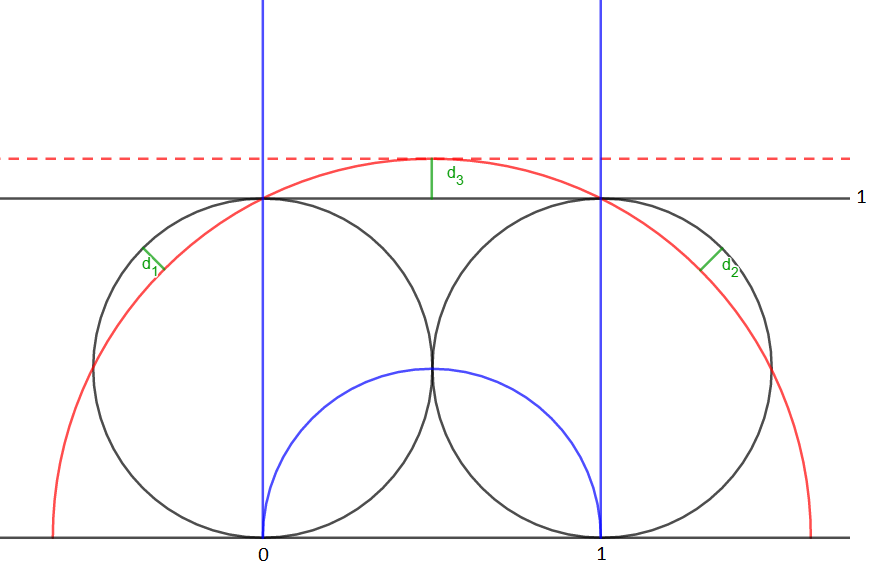
\includegraphics[width=0.2\linewidth]{pic6}
	\end{figure}
	\begin{gather*}
		U_1 = (0,1) \times (0,1)\quad \varphi_1 = \operatorname{id}\\
		U_2 = \left[0, \frac{1}{2}\right) \times (0,1)\quad \varphi_2 = \operatorname{id}\\
		U_3 = \left[\frac{1}{2},1\right] \times (0,1)\quad \varphi_3 = (x-1, 1-y)\\
		U_4 = U_2 \sqcup U_3\quad \varphi_4 |_{U_2} = \varphi_2\quad \varphi_4|_{U_3} = \varphi_3
	\end{gather*}
	Рассмотрим последовательность $U_1, U_2, U_3, U_4$
	\begin{gather*}
		\varphi_{12} = \varphi_{2} \circ \varphi_{1}^{-1} = \operatorname{id}\quad |J_{12}|>0\\
		\varphi_{24} = \varphi_{4} \circ \varphi_{2}^{-1} = \varphi_{4} = \varphi_{1}\quad |J_{24}|>0\quad \text{ так как } \varphi_{24} \text{ действует на } U_4 \cap U_2 = U_2\\
		\varphi_{42} = \varphi_{3} \circ \varphi_{4}^{-1} = \varphi_{3} \circ \varphi_{3}^{-1} = \operatorname{id}\quad |J_{43}| > 0\\
		\varphi_{31} = \varphi_{1} \circ \varphi_{3}^{-1}\\
		\varphi_{1} \circ \varphi_{3}^{-1}(x,y) = \varphi_{1}(x+1,1-y) = (x+1,1-y)\\
		|J_{31}| = 
		\begin{bmatrix}
			1 & 0 \\ 0 & -1
		\end{bmatrix}
		< 0
	\end{gather*}
	Следовательно цепочка карт противоречива
	\vskip 0.3in

	\begin{figure}[!h]
		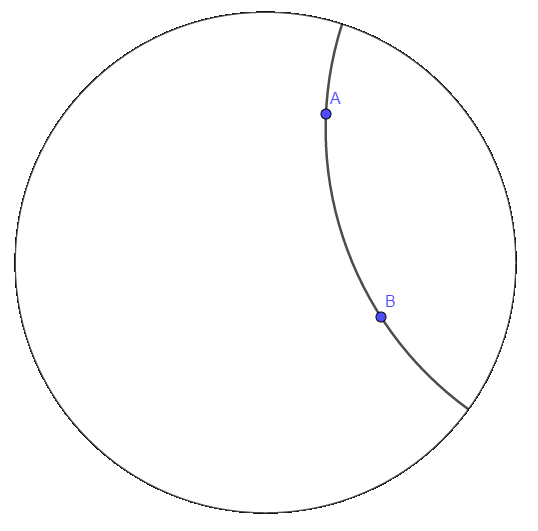
\includegraphics[width=0.2\linewidth]{pic7}
	\end{figure}
	\begin{enumerate}
	\item[(1)]
		\begin{gather*}
		U_1 = (0,1) \times (0,1)\quad \varphi = \operatorname{id}\\
		V_1 = \left[0,\frac{1}{2}\right) \times \left[0,\frac{1}{2}\right)\\
		V_2 = \left[0,\frac{1}{2}\right) \times \left(\frac{1}{2}, 1\right]
		\end{gather*}
	\item[(2)]
		\begin{gather*}
		U_2 = V_1 \cup V_2\\
		\varphi_2|_{V_1} = (x+\frac{1}{2}, y+\frac{1}{2})\\
		\varphi_2|_{V_2} = (x+\frac{1}{2}, y-\frac{1}{2})\\
		W_1 = \left(\frac{1}{2},1\right] \times \left[0,\frac{1}{2}\right)\\
		W_2 = \left(\frac{1}{2}, 1\right] \times \left(\frac{1}{2},1\right]
		\end{gather*}
	\item[(3)]
		\begin{gather*}
		U_3 = W_1 \cup W_2\\
		\varphi_3|_{W_1} = (x-\frac{1}{2}, \frac{1}{2}-y)\\
		\varphi_3|_{W_2} = (x-\frac{1}{2}, \frac{3}{2}-y)
		\end{gather*}
	\item[(4)]
		\begin{gather*}
		U_4 = U_2 \cup U_3\\
		\varphi_4|_{U_2} = \varphi_2\\
		\varphi_4|_{U_3} = \varphi_3
		\end{gather*}
	\end{enumerate}
	Рассмотрим цепочку $U_1,U_2,U_4,U_3$
	\begin{gather*}
	\varphi_{12} = \varphi_{2} \circ \varphi_{1}^{-1} = \varphi_{2}\quad |J_12|>0\\
	\varphi_{24} = \varphi_{4} \circ \varphi_{2}^{-1} = \varphi_{2}\circ\varphi_{2}^{-1}=\operatorname{id}\quad |J_{24}|>0\\
	\varphi_{43} = \varphi_{3} \circ \varphi_{4}^{-1} = \varphi_{3}^{-1} \circ \varphi_{3} = \operatorname{id}\quad |J_{43}|>0\\
	\varphi_{31} = \varphi_{1} \circ \varphi_{3}^{-1} = \varphi_{3}^{-1} \text{ на } U_1 \cap U_3:\\
	\varphi_{3}^{-1} = (x+\frac{1}{2}, -y+\frac{1}{2})\quad |J_{31}| = 
	\begin{bmatrix}
		1 & 0 \\ 0 & -1
	\end{bmatrix}
	< 0
	\end{gather*}
	Цепочка карт противоречива

\item[(б)*]
\end{enumerate}


\subsection*{Задача 7}
	Лемма из лекции:\\
	$F: M \to N$ -- диффеоморфизм, следовательно $C(M) \to C(N)$ -- изоморфизм.\\
	Зададим на $M$ разные гладкие структуры и перепишем лемму в виде $F: M \to M$ -- диффеоморфизм, следовательно $C(M)$ на обеих структурах -- одно и то же.\\
	Докажем в обратную сторону. На первой структуре введем карты $(U,\varphi)$, на второй $(V, \psi)$\\
	\begin{tikzcd}
		U \cap V \arrow{dr}{f} \arrow{r}{\psi} \arrow{d}{\varphi} &
			\mathbb{R}^n \arrow{dl}[crossing over]{F} \arrow{d}{\hat{f}}\\
		\mathbb{R}^n \arrow{r}{\tilde{f}}&
			\mathbb{R}
	\end{tikzcd}\\
	Пусть $\tilde{f}$ отдает $i$ координату, это гладкое отображение. Тогда $f := \tilde{f} \circ \varphi$ -- гладкое в 1й структуре, но тогда и во второй тоже гладкое, а следовательно $\exists$ гладкое $\hat{f}: f = \hat{f} \circ \psi$.\\
	Тогда $\hat{f} = \tilde{f} \circ F$, так как $\tilde{f}$ -- взятие $i$-й координаты, то $\hat{f} = F^i$ -- $i$-я координата $F$, а следовательно $F^i$ -- гладкое. Проделав такое со всеми координатами, получим, что $F$ -- гладкое, аналогично $F^{-1}$ тоже гладкое.\\
	$F = \varphi \circ \psi^{-1}$, $\varphi,\psi$ -- гомео., откуда $F$ -- биекция, а следовательно и диффеоморфизм, откуда следует, что карты согласованы и гладкие структуры совпадают.

\subsection*{Задача 8}
\begin{enumerate}
\item[(а)]
	Рассмотрим кривую 
	\begin{gather*}
		\beta: (-\pi, \pi) \to \mathbb{R}^2\\
		\beta(t) = (\sin 2t, \sin t)
	\end{gather*}
	Ее же можно также задать как
	\begin{gather*}
		x^2 = 4y^2(1-y^2)
	\end{gather*}
	Тогда заметим, что $\beta$ -- инъективное погружение, так как $\beta'(t) \ne (0,0)$\\
	По определению функция является вложением, если выполнены следующие факты:
	\begin{enumerate}
	\item[(1)] функция инъективна
	\item[(2)] является погружением
	\item[(3)] гомео на образ в индуцированной топологии
	\end{enumerate}
	Теперь заметим, что $\beta((-\pi, \pi))$ -- компактно в $\mathbb{R}^2$, а $(-\pi, \pi)$ не является компактом, следовательно условие (3) не выполнено
	
\item[(б)]
	Рассмотрим $f: \mathbb{R} \to \mathbb{R}^2$ -- гладкое, $f(t) = (\sin 2t, \sin t)$\\
	$L = \beta^{-1}(-\pi,\pi)$ -- подмногообразие $\mathbb{R}^2$ с топологией и гладкой структурой индуцированной $\beta^{-1}$.\\
	$f(\mathbb{R}) \subset \beta(L)$
	\begin{figure}[!h]
		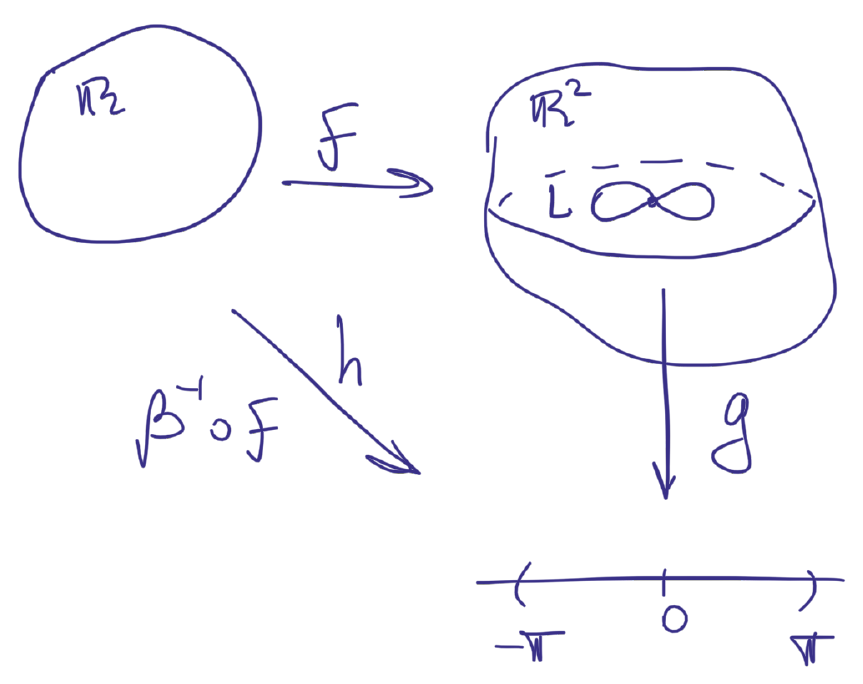
\includegraphics[width=0.4\linewidth]{pic10}
	\end{figure}
	$\beta \circ f(t)$ не является непрерывной в $t = \pi$
\end{enumerate}



\subsection*{Задача 9*}


\subsection*{Задача 10*}
\begin{comment}
	Рассмотрим конечный набор из $k$ локальных карт $\{U_i,\varphi_i = (\varphi_i^{1},\ldots,\varphi_i^{m})\}$ покрывающий многообразие $M$. Выберем карты так, чтобы образ $\varphi_i(U_i) \subset \mathbb{R}^{m}$ не содержал $0$. Так как пересечения $U_i \cap U_j$ открыты, то мы можем найти меньшие множества $V_i \subset U_i$ такие, что $\bigcup\limits_{i} V_i = M$. Рассмотрим тогда гладкую функцию $f_i \mathbb{R}^m \to \mathbb{R}$, равную $1$ на $V_i$ и $0$ вне $U_i$. Продолжим $\varphi_i^{j}|_{V_i}$ до гладких $\psi_i^{j}: M \to \mathbb{R}$, $\psi_i^{j} = f_i(x)\varphi_i^{j}(x)$ при $x \in U_i$ и $\psi_i^{j}(x) = 0$ при $x \in M\backslash U_i$.\\
	Докажем что набор функций $\{\psi_i^{j}(i = 1, \ldots, k;\ j = 1,\ldots,m), f_i(i = 1,\ldots,k)\}$ задает вложение $F:M \to \mathbb{R}^{km+k}$. Пусть $x \in V_i$, тогда $\operatorname{rang}(dF_x) \leqslant \dim M = m$. Также заметим, что $\psi_i^{j}$ на $U_i$ совпадает с некоторыми координатами функции $F$ и поэтому $\operatorname{rang}(dF) \geqslant \operatorname{rang}(d\psi_i) = \operatorname{rang}(d\varphi_i) = m$, откуда $\operatorname{rang}(dF) = m$ в каждой точке $M$, а следовательно $F$ -- погружение.\\
	Докажем что $F$ инъективно, пусть $a_1 \ne a_2$ и $a_1 \in V_i$. Тогда $f_i(a_1) = 1$, если $f_i(a_2)\ne 1$, то $F(a_1) \ne F(a_2)$, если $f_i(a_2) = 1$, то $a_2 \in U_i$ и $\psi_i(a_1) = \varphi_i(a_1) \ne \varphi_i(a_2) = \psi_i(a_2)$, следовательно $F(a_1) \ne F(a_2)$.
\end{comment}

